\chapter{Many fiber simulations} \label{chap:four}

\section{Proof of concept}

	\begin{table}
		\rowcolors{1}{}{lightgray}
		\centering
		\caption{Reference parameters for all simulations presented in this chapter. Note that $n_j$ and $\delta_j$ are functions of $j$. For each $j$, $n_j$ is constant and $\delta_j$ is linear. \label{table:manyfiber_reference}}
		\begin{tabular}{lcrclcr}
			$m$ & = & 10 & \hspace{1in} & $\ell_-$ & = & 1 \\
			$n_j$ & = & 96 & & $\ell_+$ & = & 1 \\
			$n_+$ & = & 360 & & $\ell$ & = & 1 \\
			$n_-$ & = & 310 & & $\gamma$ & = & 100 \\
			$x^{(-)}$ & = & -110 & & $\beta$ & = & 10 \\
			$y^{(-)}$ & = & 0 & & $\eps_-$ & = & 0.1 \\
			$x^{(+)}$ & = & -160 & & $\eps_+$ & = & 1 \\
			$y^{(+)}$ & = & 110 & & $\eps$ & = & 0.1 \\
			$\delta_j$ & = & 10$j$ & & $\sigma$ & = & 1
		\end{tabular}
	\end{table}

	In Chapter~\ref{chap:three} we discussed three different simulation experiments. Here we look at the compression experiment with ten fibers. As before we have a set of reference parameters (see Table~\ref{table:manyfiber_reference}). We run the compression experiment for the reference parameters and three variations of the parameters, specifically varying $\beta$, $\gamma$, and $\eps_+$.

	\begin{figure}
		\begin{center}
			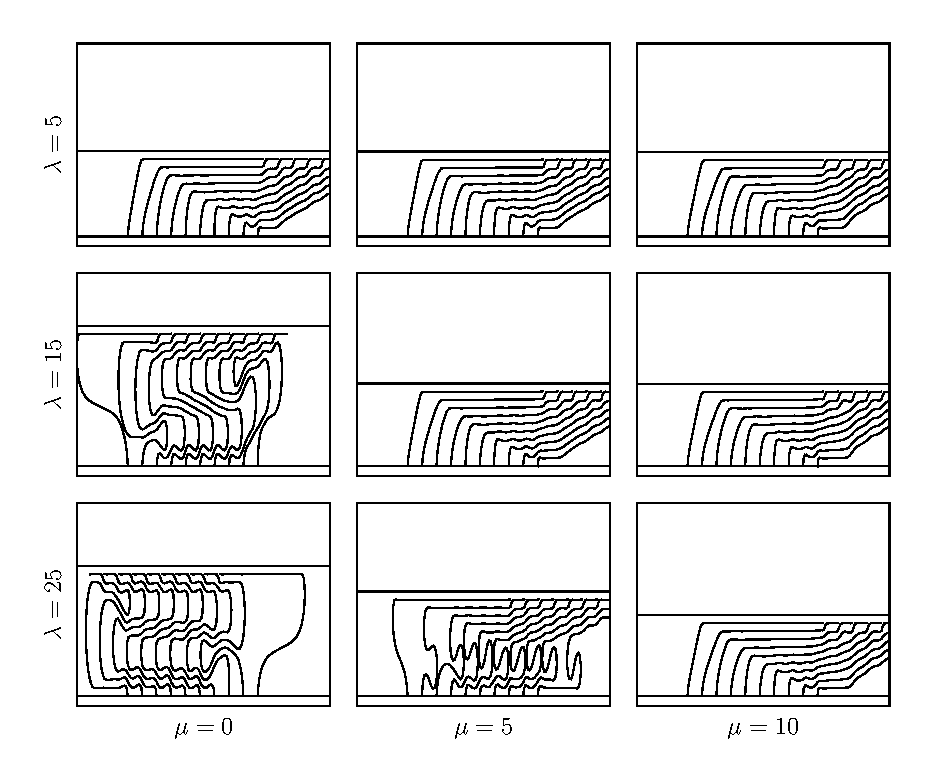
\includegraphics[scale=1]{./fig/ch4/grid.eps}
		\end{center}		
		\caption{Equilibrium configurations of ten fibers with 96 particles each for varying loads. The top left plot is a configuration with a load of $\lambda = 5$ and $\mu = 0$. The configurations to the right and below correspond to an increasing $\mu$ and increasing $\lambda$ respectively. All configurations use the reference parameters in Table~\ref{table:manyfiber_reference}.
		\label{fig:grid}}
	\end{figure}
	
	We consider nine simulations with values of $\lambda = 5, 15, 25$ and $\mu = 0, 5, 10$. In Figure~\ref{fig:grid} we see a high level view of each simulation for the reference parameters. Keeping the horizontal component of the load zero, we see an increase in bends of all ten fibers as we increase $\lambda$. One explanation for this is that the torsional and extensible springs do not have enough time to slide along the top substrate and align to it. As the magnitude of the vertical component of the load is increased the fibers become more likely to buckle. 
	
	If we increase the horizontal component of the load the story changes. We are able to maintain the aligned compressed configuration for larger magnitudes of the load if the horizontal component is sufficiently large. It would seem that the ratio between vertical and horizontal component for the reference parameters is the deciding factor for whether or not fibers will buckle. This is analogous to crushed configurations for $\theta$ near $0$\textdegree\ and flattened configurations for increased $\theta$ in Chapter~\ref{chap:three} 

	\begin{figure}
		\begin{center}
			\includegraphics[scale=1]{./fig/ch4/grid_b100.eps}
		\end{center}		
		\caption{Equilibrium configurations of varying loads. All configurations are directly comparable to Figure~\ref{fig:grid} with the exception that $\beta = 100$.
		\label{fig:grid_b100}}
	\end{figure}

	In Figure~\ref{fig:grid_b100} we increase $\beta$ to one hundred. This is an order of magnitude increase from the reference parameters and it prevents buckling at all selected loads. Qualitatively there is no discernible difference in any of the nine simulations with the one exception that the fibers buckle to the left with no horizontal component of the load. The ``crushed'' configurations of the reference parameters no longer occur similar to the single fiber situation. Although the single bend of a fiber for a single fiber only occured for $\beta=1000$ perhaps the inter-fiber vdW interaction reinforces this configuration.
	
	\begin{figure}
		\begin{center}
			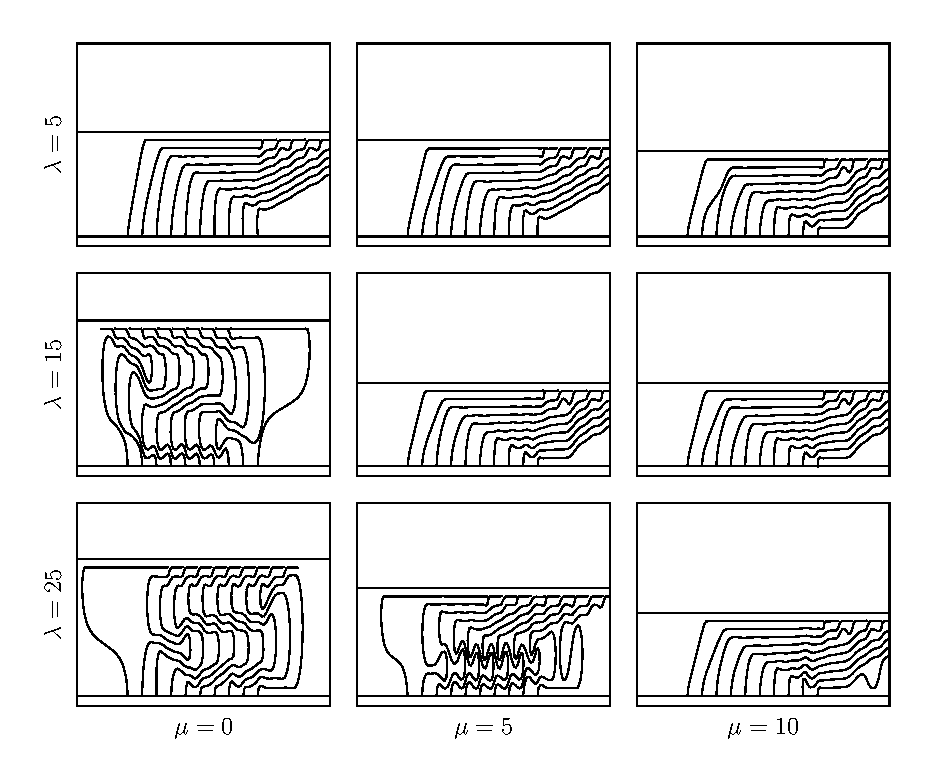
\includegraphics[scale=1]{./fig/ch4/grid_g1000.eps}
		\end{center}		
		\caption{Equilibrium configurations of varying loads. All configurations are directly comparable to Figure~\ref{fig:grid} with the exception that $\gamma = 1000$.
		\label{fig:grid_g1000}}
	\end{figure}
	
	We observe that the increase in the torsional spring strength prevents buckling to happen anywhere except the junction between the fiber and the substrate. On the other hand when we increase the extensible spring constant by an order of magnitude the buckling patterns are the same as those observed for the reference parameters. Comparing Figure~\ref{fig:grid_g1000} to Figure~\ref{fig:grid}, the same kinds of configurations are present in both. With $\gamma$ sufficiently large and vdW sufficiently weak, further increasing $\gamma$ plays a negligible role because the distance between particles on a fiber is already close to $\ell$.
	
	\begin{figure}
		\begin{center}
			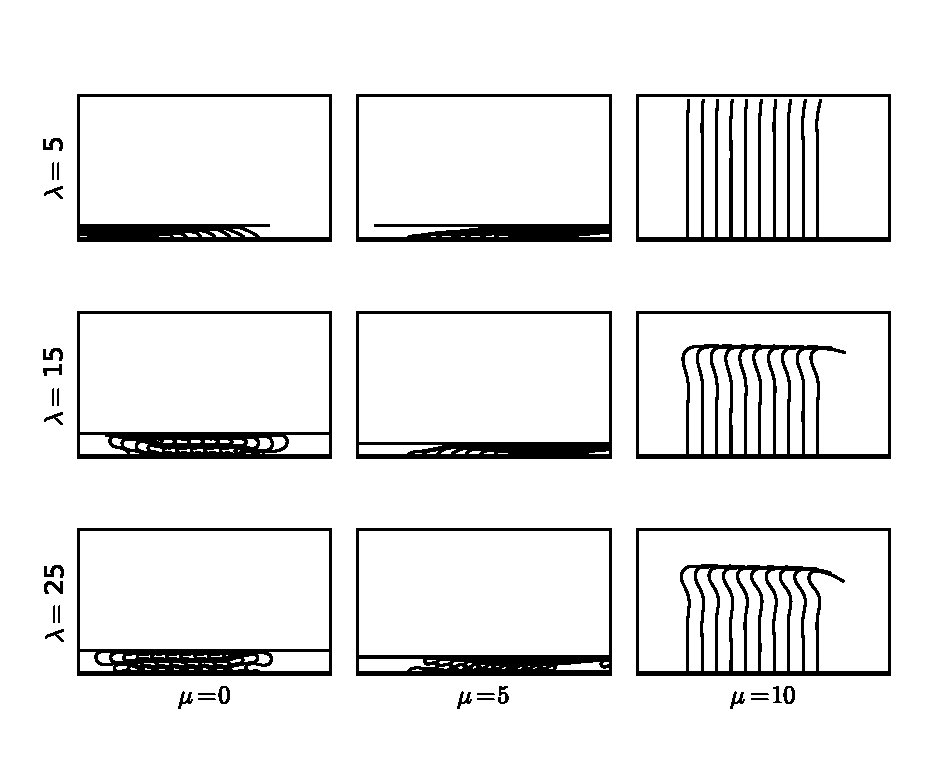
\includegraphics[scale=1]{./fig/ch4/grid_et0.1.eps}
		\end{center}		
		\caption{Equilibrium configurations of varying loads. All configurations are directly comparable to Figure~\ref{fig:grid} with the exception that $\eps_+ = 0.1$.
		\label{fig:grid_et0.1}}
	\end{figure}

	Next, consider the situation when all vdW strengths in the system are the same. In Figure~\ref{fig:grid_et0.1} we reduce $\eps_+$ to 0.1 and present the results for nine different loads while keeping the rest of the parameters equal to the reference values. For $\mu = 0$ or $5$ the configurations are comparable. We further observe that the horizontal component of the load can be strong enough to cause the top substrate to slide off the fibers overpowering the vdW interaction. This happens for all values of the vertical component of the load that we have considered when $\mu = 10$.
	
	Although we focus primarily on the model for only a single fiber it was designed for arbitrarily many and arbitrarily large fibers. Investigating the single fiber case does give us some insight into how many fibers will behave as well.

\section{Future work}

In Chapter~\ref{chap:three} we explored three numerical experiments.
The compression experiment was explored briefly here, but the detachment experiment was not explored at all.
Overcoming numerical difficulties connected to much larger sizes of the simulation for both compression and detachment is a significant issue that we have not addressed.
Coarse-grained approaches like molecular dynamics approaches scale with parallelization very well and that could be used to evolve large scale systems over long time steps.

The single fiber setup presented in Chapter~\ref{chap:three} we varied two parameters for each plot.
This approach gave interesting results for the specific parameters of interest ($\lambda$ and $\mu$) but it does not as effectively explore the rest of the parameter space.
Likewise, many of the arguments for the behavior of the system are either by direct example or from numerical trends of the simulations.
There are four modes of detachment discovered, simple sliding, wave propagated sliding, brute forcing, and unzipping.
It appears that are only really two modes of detachment, sliding and unzipping, but this is not entirely clear from numerical experiment alone.

For many fibers it is more difficult to explore the parameter space in a way to categorize exact equilibrium configurations simply because of the number of particles.
However, a sensitivity analysis of the parameter space could give insight into the behavior and a detachment experiment with many fibers would demonstrate how the detachment modes behave with inter-fiber adhesion.
Applying the model to physical situations is out of the scope of this work but parameterization of ``bead-spring'' models of similar kind have been used to some success to model CNTs.

